\chapter{Experiments}
\label{Experiments}
In experiments that focus on measuring the quality assessment of synthetic images (for depth estimation task in \ref{Expt_1} and for HX4-PET synthesis task \ref{Expt_2}), we considered Pix2Pix as an ``upperbound" image translation method, and measured the degree to which the performances of CycleGAN-naive and CycleGAN-balanced approach this upperbound. Pix2Pix was expected to perform better due to its paired (supervised) training.



%%%%%%%%%%%%%%%%%%%%%%%%%%%%%%%%%%%%%%%%%%%%%%%%%%%%%%%%%%%%%%%%%%%%%%%%%%%%%%%%%%%%%%%%%%%%%%%%%%%%%%%%%%%%%%%%%%%%%%%%%%%%%%%%%%%%%%%%%%%%%%%
\section{Experiment 1: Testing the GANs on Depth Estimation Problem}
\label{Expt_1}


% ---------------------------
\subsection{Experiment Setup}

\subsubsection{Training configuration}
The curated dataset for the depth estimation task is a subset of the original ClearGrasp dataset (see \ref{ClearGrasp_Depth_Estimation}). During training, images of all three modalities were first rescaled to size 512$\times$256 and normalized to [-1, 1] range.  For Pix2Pix, $\lambda$ value 100 for the element-wise loss was observed to produce good results, whereas a $\lambda$ of 10 was used for the cycle-consistency loss in both CycleGANs. Similar to the optimizer configuration used in the original Pix2Pix and CycleGAN papers \cite{isola2017image, zhu2017unpaired}, we use Adam optimizer with moment parameter settings $\beta_1$=0.5 and $\beta_2$=0.999. Initial learning rate value of 0.0002 was used for the generators and 0.0001 for the discriminators. Each model was trained with a batch size of 1 on full images for 50 epochs. The learning rates were fixed for the first 25 epochs and then linearly decayed to 0 over the next 25 epochs. Model validation was performed after each epoch. Training was performed on an NVIDIA Tesla P100 SXM2 (16 GB) GPU hardware provided as part of the RWTH Aachen Compute Cluster, and the training time for 2D Pix2Pix, CycleGAN-naive and CycleGAN-balanced models were approximately 2 hours, 4 hours and 5 hours respectively.

\subsubsection{Evaluation settings}
Pixel-wise mean-squared error (MSE) between the synthetic and ground-truth depthmaps was used as the evaluation metric. Before computing the MSE, the image intensities were converted back to their original depth representation in meters.


% -------------------------------
\subsection{Results and Analysis}
Table \ref{tab:rcleargrasp_quant} reports the MSE values for each of the models' predictions on the validation set. Pix2Pix was the best performing and most robust model, as expected, setting the performance upper-bound among the three models. CycleGAN-naive performed the worst, whereas CycleGAN-balanced achieved comparatively better results. 

\begin{table}[h!]
    \small
    \centering
    \begin{tabular}{ccccccc}
        \textbf{Method} & \textbf{MSE} \\
        \hline
        Pix2Pix    & \textbf{0.004} $\pm$ 0.005 \\
        CycleGAN-naive    & 0.192 $\pm$ 0.253 \\
        CycleGAN-balanced    & 0.147 $\pm$ 0.170 \\
    \end{tabular}
    \caption{Mean-squared error (expressed as meter$^2$) over the curated validation set from the ClearGrasp dataset.}
    \label{tab:rcleargrasp_quant}
\end{table}

\begin{figure}[h!]
    \centering
    \makebox[\textwidth][c]
    {   
        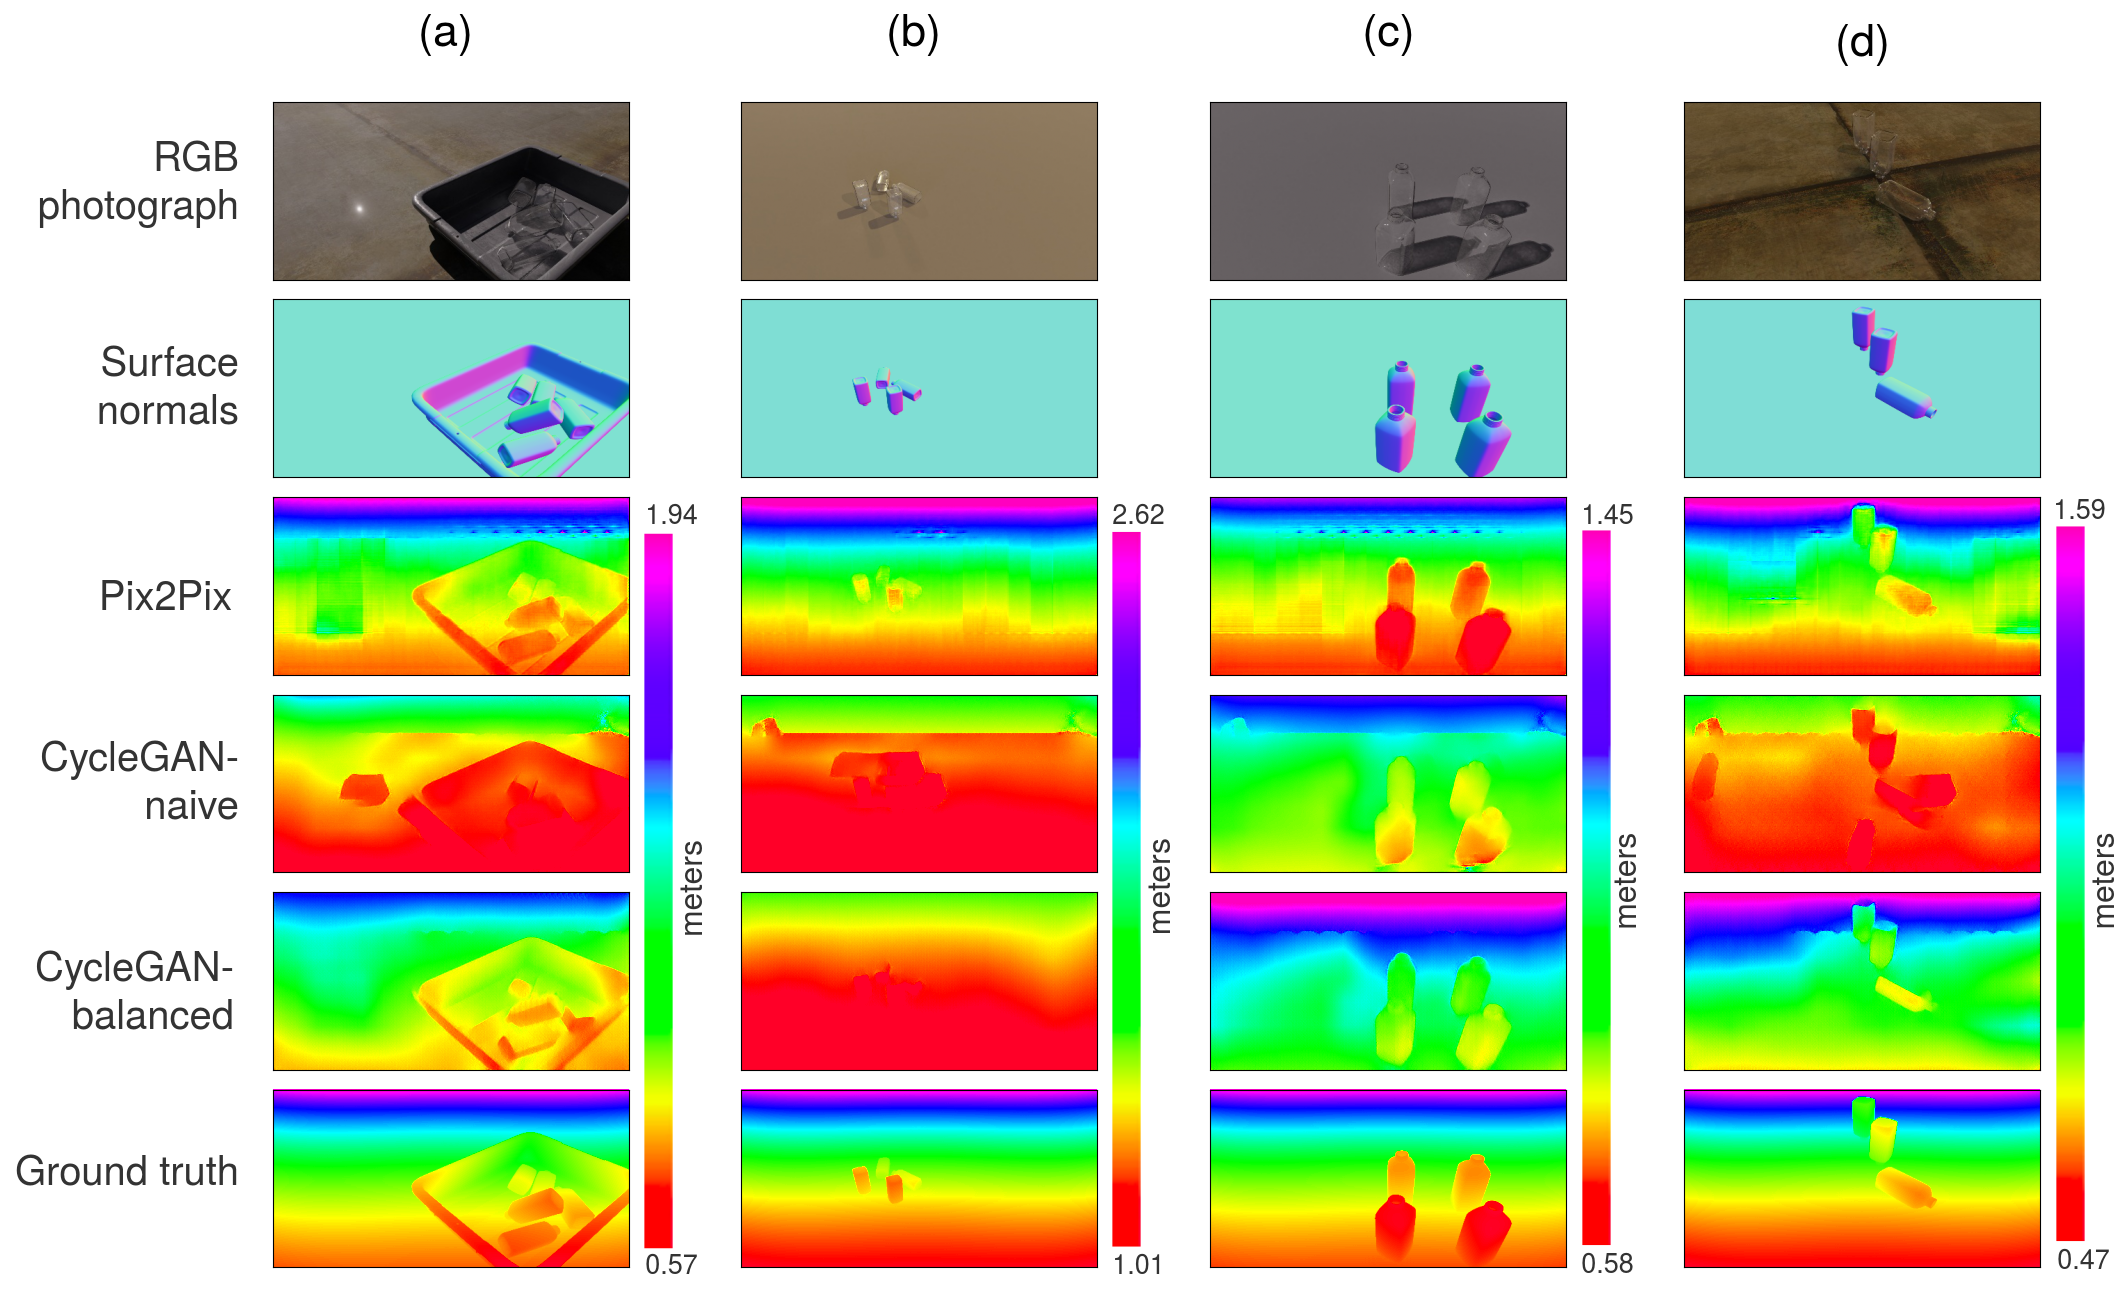
\includegraphics[width=1.1\linewidth]{figures/Expt_1/Cleargrasp_Results-viz.png}
    }
    \caption{Selected validation samples chosen to highlight the challenges in input data –- (a) a nearby tray containing transparent objects and a reflection on the floor, (b) distant objects, (c) objects casting strong shadows, and (d) a strong cross-shaped pattern on the floor. Pix2Pix model estimated the depth of the transparent objects, other objects and the floor very close to the ground truth. CycleGAN-naive produced depthmaps with heavy artifacts, which were absent in case of CycleGAN-balanced, notably in (a) and (d).}
    \label{fig:cleargrasp_qual}
\end{figure}

Figure \ref{fig:cleargrasp_qual} shows qualitative results showing samples that are representative of the MSE measurements. ... 



%%%%%%%%%%%%%%%%%%%%%%%%%%%%%%%%%%%%%%%%%%%%%%%%%%%%%%%%%%%%%%%%%%%%%%%%%%%%%%%%%%%%%%%%%%%%%%%%%%%%%%%%%%%%%%%%%%%%%%%%%%%%%%%%%%%%%%%%%%%%%%%
\section{Experiment 2: Image Quality Metrics For Synthetic HX4-PET Assessment}
\label{Expt_2}


% ---------------------------
\subsection{Experiment Setup}

\subsubsection{Training configuration}

Because a patch-based training approach is used that involves random sampling (see \ref{training_pipeline}), the notion of an ``epoch" doesn't exist here. Instead, the number of iterations is used as a measure of training duration, where an iteration corresponds to a forward pass followed by the update of weights of all networks in the GAN system. In our experiments, we train each GAN model for 60,000 iterations. 
The scaling factor for the element-wise loss in Pix2Pix ($\lambda$ in Equation \ref{eq:pix2pix_loss_components}) is set to 10, and the cycle-consistency loss for CycleGAN is scaled by 10 as well ($\lambda$ in Equation \ref{eq:cyclegan_naive_loss_components}). Similar to the optimizer configuration used in the original papers \cite{isola2017image, zhu2017unpaired}, we use Adam optimizer with moment parameter settings $\beta_1$=0.5 and $\beta_2$=0.999. Initial learning rates 0.0002 for the generators and 0.0001 for the discriminators are used during the first 30,000 iterations and are linearly decayed to 0 over the next 30,000 iterations. Model validation is performed every 1000 iterations. All models were trained with batch size 1.

The GANs and the model training pipeline were implemented entirely in \textit{PyTorch}. Training was performed on an NVIDIA Tesla V100 SXM2 (32 GB) GPU provided as part of the Data Science Research Infrastructure (DSRI) \footnote{\url{https://maastrichtu-ids.github.io/dsri-documentation/}} from Maastricht University. The training time for Pix2Pix, CycleGAN-naive and CycleGAN-balanced were 9.5 hours, 13 hours and 15.25 hours, respectively. 


\subsubsection{Evaluation settings}


% ------------------------------------------------------------------
\subsection{Results and Analysis 1: Evaluating Fully Trained Models}


% -----------------------------------------------------------------------------------
\subsection{Results and Analysis 2: To Analysis of Model Convergence during Training}



%%%%%%%%%%%%%%%%%%%%%%%%%%%%%%%%%%%%%%%%%%%%%%%%%%%%%%%%%%%%%%%%%%%%%%%%%%%%%%%%%%%%%%%%%%%%%%%%%%%%%%%%%%%%%%%%%%%%%%%%%%%%%%%%%%%%%%%%%%%%%%%
\section{Experiment 3: Application-specific Downstream Tasks}
\label{Expt_3}


% ---------------------------
\subsection{Experiment Setup}


% -------------------------------
\subsection{Results and Analysis}
